\documentclass[11pt,a4paper,]{article}
\usepackage{lmodern}

\usepackage{amssymb,amsmath}
\usepackage{ifxetex,ifluatex}
\usepackage{fixltx2e} % provides \textsubscript
\ifnum 0\ifxetex 1\fi\ifluatex 1\fi=0 % if pdftex
  \usepackage[T1]{fontenc}
  \usepackage[utf8]{inputenc}
\else % if luatex or xelatex
  \usepackage{unicode-math}
  \defaultfontfeatures{Ligatures=TeX,Scale=MatchLowercase}
\fi
% use upquote if available, for straight quotes in verbatim environments
\IfFileExists{upquote.sty}{\usepackage{upquote}}{}
% use microtype if available
\IfFileExists{microtype.sty}{%
\usepackage[]{microtype}
\UseMicrotypeSet[protrusion]{basicmath} % disable protrusion for tt fonts
}{}
\PassOptionsToPackage{hyphens}{url} % url is loaded by hyperref
\usepackage[unicode=true]{hyperref}
\hypersetup{
            pdftitle={Immigration Report},
            pdfborder={0 0 0},
            breaklinks=true}
\urlstyle{same}  % don't use monospace font for urls
\usepackage{geometry}
\geometry{a4paper, centering, text={16cm,24cm}}
\usepackage[style=authoryear-comp,]{biblatex}
\addbibresource{references.bib}
\usepackage{longtable,booktabs}
% Fix footnotes in tables (requires footnote package)
\IfFileExists{footnote.sty}{\usepackage{footnote}\makesavenoteenv{long table}}{}
\usepackage{graphicx,grffile}
\makeatletter
\def\maxwidth{\ifdim\Gin@nat@width>\linewidth\linewidth\else\Gin@nat@width\fi}
\def\maxheight{\ifdim\Gin@nat@height>\textheight\textheight\else\Gin@nat@height\fi}
\makeatother
% Scale images if necessary, so that they will not overflow the page
% margins by default, and it is still possible to overwrite the defaults
% using explicit options in \includegraphics[width, height, ...]{}
\setkeys{Gin}{width=\maxwidth,height=\maxheight,keepaspectratio}
\IfFileExists{parskip.sty}{%
\usepackage{parskip}
}{% else
\setlength{\parindent}{0pt}
\setlength{\parskip}{6pt plus 2pt minus 1pt}
}
\setlength{\emergencystretch}{3em}  % prevent overfull lines
\providecommand{\tightlist}{%
  \setlength{\itemsep}{0pt}\setlength{\parskip}{0pt}}
\setcounter{secnumdepth}{5}

% set default figure placement to htbp
\makeatletter
\def\fps@figure{htbp}
\makeatother


\title{Immigration Report}

%% MONASH STUFF

%% CAPTIONS
\RequirePackage{caption}
\DeclareCaptionStyle{italic}[justification=centering]
 {labelfont={bf},textfont={it},labelsep=colon}
\captionsetup[figure]{style=italic,format=hang,singlelinecheck=true}
\captionsetup[table]{style=italic,format=hang,singlelinecheck=true}


%% FONT
\RequirePackage{bera}
\RequirePackage[charter,expert,sfscaled]{mathdesign}
\RequirePackage{fontawesome}

%% HEADERS AND FOOTERS
\RequirePackage{fancyhdr}
\pagestyle{fancy}
\rfoot{\Large\sffamily\raisebox{-0.1cm}{\textbf{\thepage}}}
\makeatletter
\lhead{\textsf{\expandafter{\@title}}}
\makeatother
\rhead{}
\cfoot{}
\setlength{\headheight}{15pt}
\renewcommand{\headrulewidth}{0.4pt}
\renewcommand{\footrulewidth}{0.4pt}
\fancypagestyle{plain}{%
\fancyhf{} % clear all header and footer fields
\fancyfoot[C]{\sffamily\thepage} % except the center
\renewcommand{\headrulewidth}{0pt}
\renewcommand{\footrulewidth}{0pt}}

%% MATHS
\RequirePackage{bm,amsmath}
\allowdisplaybreaks

%% GRAPHICS
\RequirePackage{graphicx}
\setcounter{topnumber}{2}
\setcounter{bottomnumber}{2}
\setcounter{totalnumber}{4}
\renewcommand{\topfraction}{0.85}
\renewcommand{\bottomfraction}{0.85}
\renewcommand{\textfraction}{0.15}
\renewcommand{\floatpagefraction}{0.8}


%\RequirePackage[section]{placeins}

%% SECTION TITLES


%% SECTION TITLES (NEW: Changing sections and subsections color)
\RequirePackage[compact,sf,bf]{titlesec}
\titleformat*{\section}{\Large\sf\bfseries\color[rgb]{0.8, 0.7, 0.1 }}
\titleformat*{\subsection}{\large\sf\bfseries\color[rgb]{0.8, 0.7, 0.1 }}
\titleformat*{\subsubsection}{\sf\bfseries\color[rgb]{0.8, 0.7, 0.1 }}
\titlespacing{\section}{0pt}{2ex}{.5ex}
\titlespacing{\subsection}{0pt}{1.5ex}{0ex}
\titlespacing{\subsubsection}{0pt}{.5ex}{0ex}


%% TITLE PAGE
\def\Date{\number\day}
\def\Month{\ifcase\month\or
 January\or February\or March\or April\or May\or June\or
 July\or August\or September\or October\or November\or December\fi}
\def\Year{\number\year}

%% LINE AND PAGE BREAKING
\sloppy
\clubpenalty = 10000
\widowpenalty = 10000
\brokenpenalty = 10000
\RequirePackage{microtype}

%% PARAGRAPH BREAKS
\setlength{\parskip}{1.4ex}
\setlength{\parindent}{0em}

%% HYPERLINKS
\RequirePackage{xcolor} % Needed for links
\definecolor{darkblue}{rgb}{0,0,.6}
\RequirePackage{url}

\makeatletter
\@ifpackageloaded{hyperref}{}{\RequirePackage{hyperref}}
\makeatother
\hypersetup{
     citecolor=0 0 0,
     breaklinks=true,
     bookmarksopen=true,
     bookmarksnumbered=true,
     linkcolor=darkblue,
     urlcolor=blue,
     citecolor=darkblue,
     colorlinks=true}

\usepackage[showonlyrefs]{mathtools}
\usepackage[no-weekday]{eukdate}

%% BIBLIOGRAPHY

\makeatletter
\@ifpackageloaded{biblatex}{}{\usepackage[style=authoryear-comp, backend=biber, natbib=true]{biblatex}}
\makeatother
\ExecuteBibliographyOptions{bibencoding=utf8,minnames=1,maxnames=3, maxbibnames=99,dashed=false,terseinits=true,giveninits=true,uniquename=false,uniquelist=false,doi=false, isbn=false,url=true,sortcites=false}

\DeclareFieldFormat{url}{\texttt{\url{#1}}}
\DeclareFieldFormat[article]{pages}{#1}
\DeclareFieldFormat[inproceedings]{pages}{\lowercase{pp.}#1}
\DeclareFieldFormat[incollection]{pages}{\lowercase{pp.}#1}
\DeclareFieldFormat[article]{volume}{\mkbibbold{#1}}
\DeclareFieldFormat[article]{number}{\mkbibparens{#1}}
\DeclareFieldFormat[article]{title}{\MakeCapital{#1}}
\DeclareFieldFormat[article]{url}{}
%\DeclareFieldFormat[book]{url}{}
%\DeclareFieldFormat[inbook]{url}{}
%\DeclareFieldFormat[incollection]{url}{}
%\DeclareFieldFormat[inproceedings]{url}{}
\DeclareFieldFormat[inproceedings]{title}{#1}
\DeclareFieldFormat{shorthandwidth}{#1}
%\DeclareFieldFormat{extrayear}{}
% No dot before number of articles
\usepackage{xpatch}
\xpatchbibmacro{volume+number+eid}{\setunit*{\adddot}}{}{}{}
% Remove In: for an article.
\renewbibmacro{in:}{%
  \ifentrytype{article}{}{%
  \printtext{\bibstring{in}\intitlepunct}}}

\AtEveryBibitem{\clearfield{month}}
\AtEveryCitekey{\clearfield{month}}

\makeatletter
\DeclareDelimFormat[cbx@textcite]{nameyeardelim}{\addspace}
\makeatother

\author{\sf\Large\textbf{ Priya Ravindra Dingorkar}\\ {\sf\large BE in Computer Enginnering, Pursing Master of Business Analytics\\[0.5cm]} \sf\Large\textbf{ Aarathy Babu}\\ {\sf\large B.Tech\\[0.5cm]} \sf\Large\textbf{ Junhao Wang}\\ {\sf\large B.Accounting\\[0.5cm]} \sf\Large\textbf{ XXX XXX (Please add your details Dilinie)}\\ {\sf\large XXX\\[0.5cm]}}

\date{\sf\Date~\Month~\Year}
\makeatletter
\lfoot{\sf Dingorkar, Babu, Wang, XXX (Please add your details Dilinie): \@date}
\makeatother


%%%% PAGE STYLE FOR FRONT PAGE OF REPORTS

\makeatletter
\def\organization#1{\gdef\@organization{#1}}
\def\telephone#1{\gdef\@telephone{#1}}
\def\email#1{\gdef\@email{#1}}
\makeatother
  \organization{Australian Government COVID19}

  \def\name{ETC5513, Group 11\newline Junhao \&\newline Aarathy \&\newline Dilinie \&\newline Priya}

  \telephone{(03) 9905 2478}

  \email{questions@company.com}                 %NEW: New email addresss

\def\webaddress{\url{http://company.com/stats/consulting/}} %NEW: URl
\def\abn{12 377 614 630}                                    % NEW: ABN
\def\logo{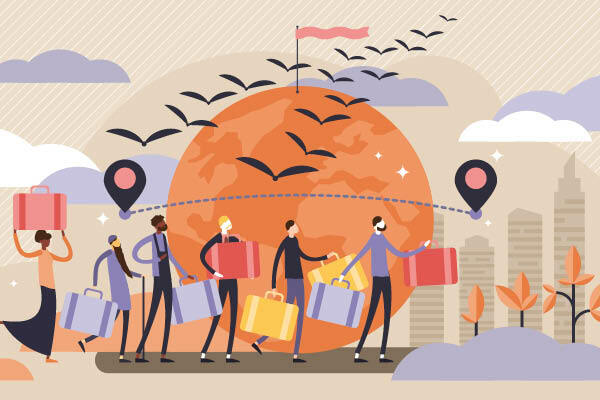
\includegraphics[width=6cm]{logo}}  %NEW: Changing logo
\def\extraspace{\vspace*{1.6cm}}
\makeatletter
\def\contactdetails{\faicon{phone} & \@telephone \\
                    \faicon{envelope} & \@email}
\makeatother

%%%% FRONT PAGE OF REPORTS

\def\reporttype{Report for}

\long\def\front#1#2#3{
\newpage
\begin{singlespacing}
\thispagestyle{empty}
\vspace*{-1.4cm}
\hspace*{-1.4cm}
\hbox to 16cm{
  \hbox to 6.5cm{\vbox to 14cm{\vbox to 25cm{
    \logo
    \vfill
    \parbox{6.3cm}{\raggedright
      \sf\color[rgb]{0.8, 0.7, 0.1 }    % NEW color 
      {\large\textbf{\name}}\par
      \vspace{.7cm}
      \tabcolsep=0.12cm\sf\small
      \begin{tabular}{@{}ll@{}}\contactdetails
      \end{tabular}
      \vspace*{0.3cm}\par
      ABN: \abn\par
    }
  }\vss}\hss}
  \hspace*{0.2cm}
  \hbox to 1cm{\vbox to 14cm{\rule{4pt}{26.8cm}\vss}\hss\hfill}  %NEW: Thicker line
  \hbox to 10cm{\vbox to 14cm{\vbox to 25cm{   
      \vspace*{3cm}\sf\raggedright
      \parbox{11cm}{\sf\raggedright\baselineskip=1.2cm
         \fontsize{24.88}{30}\color[rgb]{0, 0.29, 0.55}\sf\textbf{#1}}   % NEW: title color blue
      \par
      \vfill
      \large
      \vbox{\parskip=0.8cm #2}\par
      \vspace*{2cm}\par
      \reporttype\\[0.3cm]
      \hbox{#3}%\\[2cm]\
      \vspace*{1cm}
      {\large\sf\textbf{\Date~\Month~\Year}}
   }\vss}
  }}
\end{singlespacing}
\newpage
}

\makeatletter
\def\titlepage{\front{\expandafter{\@title}}{\@author}{\@organization}}
\makeatother

\usepackage{setspace}
\setstretch{1.5}

%% Any special functions or other packages can be loaded here.
\usepackage{booktabs}
\usepackage{longtable}
\usepackage{array}
\usepackage{multirow}
\usepackage{wrapfig}
\usepackage{float}
\usepackage{colortbl}
\usepackage{pdflscape}
\usepackage{tabu}
\usepackage{threeparttable}
\usepackage{threeparttablex}
\usepackage[normalem]{ulem}
\usepackage{makecell}
\usepackage{xcolor}


\begin{document}
\titlepage

\section*{Introduction}

This dataset provides information about OECD coutries. each file includes a number of core variables (detailed country of birth, education and sex). So our goals is to study immigrant in OECD countries and use these core variables to analyse the situation of immigrants. In this category: Priya ; Aarathy; Junhao look into the gender gap of unemployment rate, and study the relationsip between education level unemployment; Dilinie study the level of education of residents of Australia vs the duration theyve been in in Australia.

\section*{Abstract}

\section*{Methodology}

\begin{table}

\caption{\label{tab:unnamed-chunk-9}unemployment gendergap}
\centering
\begin{tabular}[t]{l|r|r|r}
\hline
country & unemployrateM & unemployrateF & unemployrateGAP\\
\hline
AUS & 4.862303 & 4.0115099 & -0.8507930\\
\hline
AUT & 5.336735 & 3.9353913 & -1.4013437\\
\hline
BEL & 4.347939 & 3.2985616 & -1.0493775\\
\hline
CAN & 5.778106 & 4.3270743 & -1.4510321\\
\hline
CHE & 3.865908 & 3.2144728 & -0.6514349\\
\hline
CHL & 4.809590 & 3.9577202 & -0.8518701\\
\hline
CZE & 2.396411 & 2.4515907 & 0.0551801\\
\hline
DEU & 2.936210 & 2.0469143 & -0.8892954\\
\hline
DNK & 2.148729 & 2.1059917 & -0.0427379\\
\hline
ESP & 10.985712 & 10.8943528 & -0.0913595\\
\hline
EST & 5.300859 & 3.4574224 & -1.8434366\\
\hline
FIN & 9.559730 & 6.8315897 & -2.7281404\\
\hline
FRA & 8.392850 & 7.8781252 & -0.5147248\\
\hline
GBR & 3.663103 & 2.8918511 & -0.7712517\\
\hline
GRC & 10.585938 & 7.4697667 & -3.1161718\\
\hline
HUN & 7.512527 & 5.7554851 & -1.7570423\\
\hline
IRL & 9.371130 & 6.6267541 & -2.7443755\\
\hline
ISL & 3.634079 & 3.1891160 & -0.4449626\\
\hline
ISR & 3.226836 & 2.9344538 & -0.2923819\\
\hline
ITA & 6.557226 & 5.1080372 & -1.4491892\\
\hline
JPN & 3.452669 & 1.6996869 & -1.7529817\\
\hline
KOR & NA & NA & NA\\
\hline
LUX & 46.543493 & 35.7410219 & -10.8024711\\
\hline
LVA & 7.869852 & 5.4260483 & -2.4438039\\
\hline
MEX & 3.497137 & 0.9523001 & -2.5448371\\
\hline
NLD & 3.881309 & 3.8180653 & -0.0632437\\
\hline
NOR & 2.147195 & 1.4721626 & -0.6750323\\
\hline
NZL & 3.579875 & 3.6812728 & 0.1013976\\
\hline
POL & 7.015866 & 5.7597853 & -1.2560810\\
\hline
PRT & 7.032256 & 5.9746734 & -1.0575825\\
\hline
SVK & 11.368361 & 8.7232843 & -2.6450766\\
\hline
SVN & 4.902322 & 4.6408436 & -0.2614786\\
\hline
SWE & 3.838277 & 3.0794607 & -0.7588166\\
\hline
TUR & 7.266447 & 4.5316713 & -2.7347755\\
\hline
USA & 3.955071 & 3.2786733 & -0.6763982\\
\hline
\end{tabular}
\end{table}

\newpage

\begin{figure}
\centering
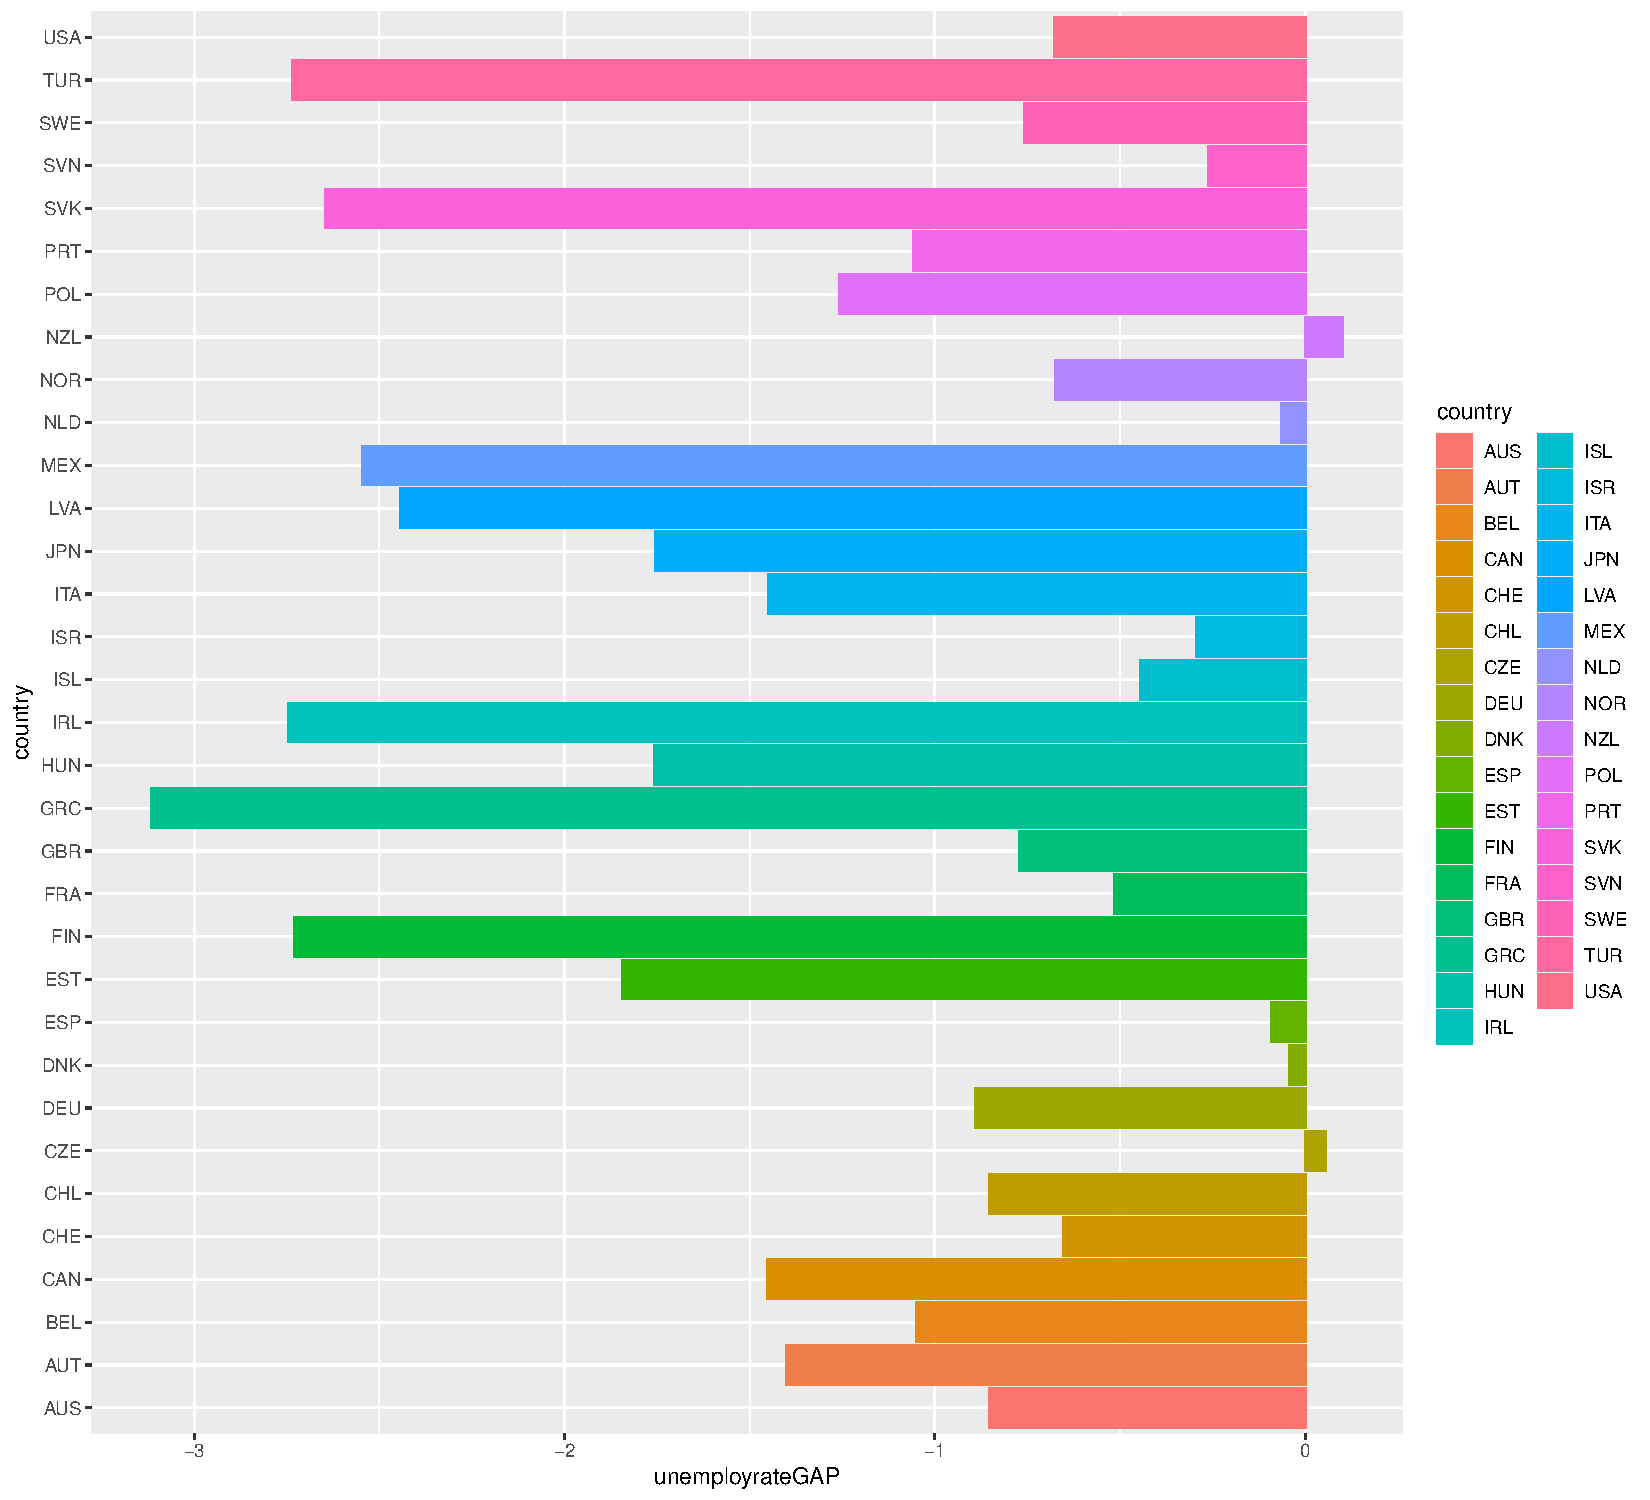
\includegraphics{ETC5513assignment4_files/figure-latex/GAP-1.pdf}
\caption{\label{fig:GAP}unemployment gender gap}
\end{figure}

Analysis:

We can draw conlusion from \ref{fig:GAP} thatGenerally speaking, gender gap in unemployment rate does exist, the unemployment rate gaps are negative in most country, this means female have lower unemployment rate than male.

\begin{table}

\caption{\label{tab:unnamed-chunk-11}unemployrate on different level of education}
\centering
\begin{tabular}[t]{l|l|r}
\hline
country & educationlevel & unemployRATE\\
\hline
AUS & high & 0.0354576\\
\hline
AUS & low & 0.0443595\\
\hline
AUS & medium & 0.0532527\\
\hline
AUS & unknown & 0.0358913\\
\hline
AUT & high & 0.0311428\\
\hline
AUT & low & 0.0701552\\
\hline
AUT & medium & 0.0457923\\
\hline
AUT & unknown & NaN\\
\hline
BEL & high & 0.0298011\\
\hline
BEL & low & 0.0431251\\
\hline
BEL & medium & 0.0461857\\
\hline
BEL & unknown & 0.0122354\\
\hline
CAN & high & 0.0452058\\
\hline
CAN & low & 0.0517304\\
\hline
CAN & medium & 0.0601727\\
\hline
CHE & high & 0.0328462\\
\hline
CHE & low & 0.0416613\\
\hline
CHE & medium & 0.0336930\\
\hline
CHL & high & 0.0179900\\
\hline
CHL & low & 0.0427796\\
\hline
CHL & medium & 0.0498058\\
\hline
CHL & unknown & 0.0527589\\
\hline
CZE & high & 0.0167868\\
\hline
CZE & low & 0.0409399\\
\hline
CZE & medium & 0.0226775\\
\hline
CZE & unknown & 0.0487416\\
\hline
DEU & high & 0.0160581\\
\hline
DEU & low & 0.0374303\\
\hline
DEU & medium & 0.0236941\\
\hline
DEU & unknown & 0.0093930\\
\hline
DNK & high & 0.0231097\\
\hline
DNK & low & 0.0177326\\
\hline
DNK & medium & 0.0225601\\
\hline
DNK & unknown & 0.0210787\\
\hline
ESP & high & 0.0880976\\
\hline
ESP & low & 0.1186934\\
\hline
ESP & medium & 0.1216533\\
\hline
ESP & unknown & 0.0000000\\
\hline
EST & high & 0.0286894\\
\hline
EST & low & 0.0441750\\
\hline
\end{tabular}
\end{table}

\pagebreak

\begin{figure}
\centering
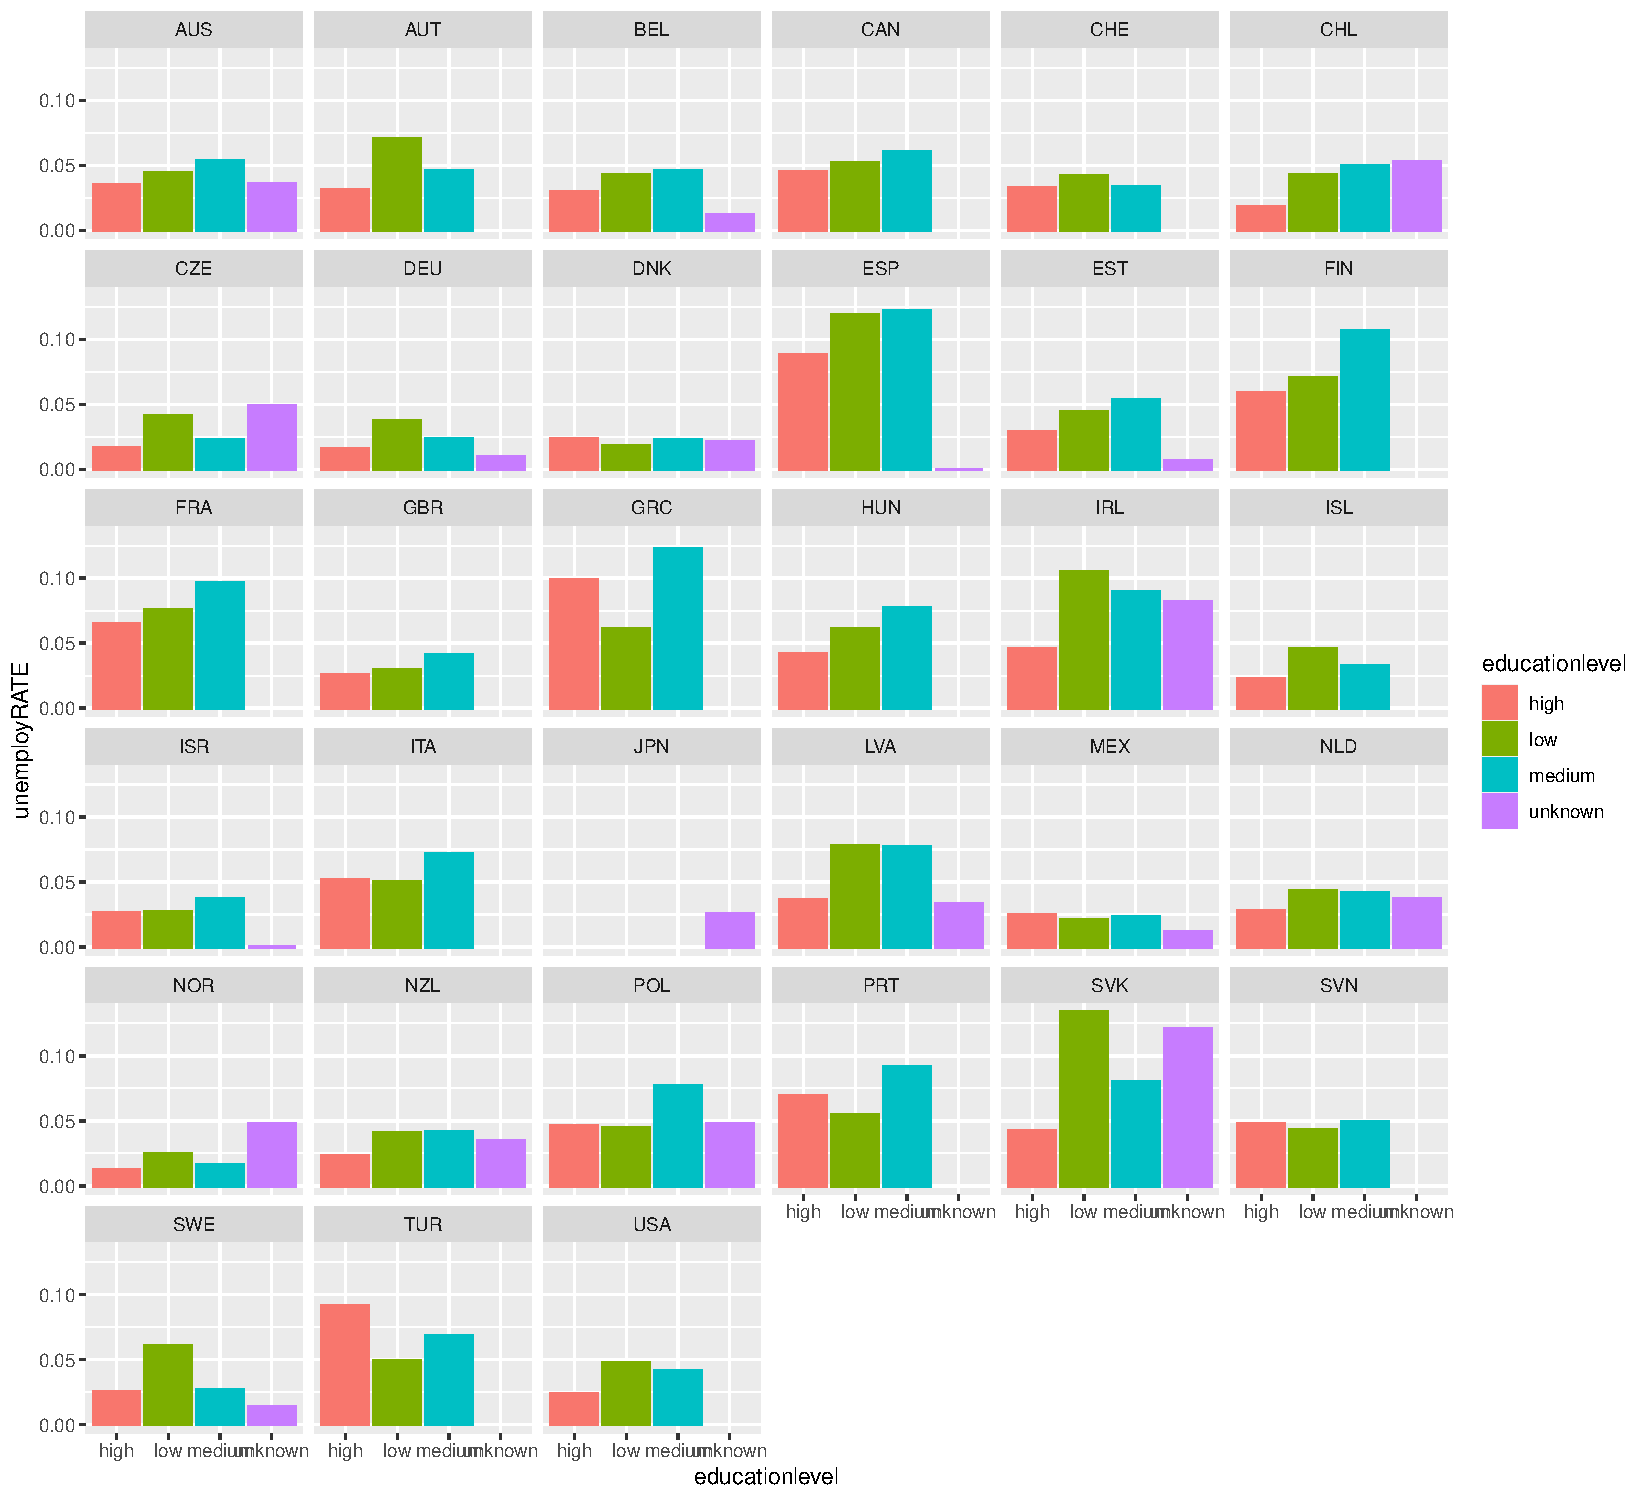
\includegraphics{ETC5513assignment4_files/figure-latex/ed_un-1.pdf}
\caption{(\#fig:ed\_un)unemployment rate among different education level}
\end{figure}

Analysis:

\ref{figure:ed_un} Generally speaking, most have lower unemployment rate compared to low education level groups, but this is not the case in TUR,PRT,RGC AND ITA.

Limitation:
There are some missing values that can influence the outcome to some extent, it is like the data I use became a smaller sample.

\printbibliography

\end{document}

